\newcommand{\lecturetitle}[1]{
  \title{01204211 Discrete Mathematics \\ #1}
  \author{Jittat Fakcharoenphol}
  \frame{\titlepage}
}
\newcommand{\Mod}{\,\bmod\,}


\newcommand\sbullet[1][.5]{\mathbin{\vcenter{\hbox{\scalebox{#1}{$\bullet$}}}}}

\lecturetitle{Lecture 9b: Nonregular languages\footnote{Based on lecture notes of {\em Models of Computation} course by Jeff Erickson.}} 
\renewcommand{\epsilon}{\varepsilon}

\newcommand{\czero}{{\mathtt 0}}
\newcommand{\cone}{{\mathtt 1}}

\begin{frame}
  \frametitle{DFA: Formal definitions}

  A {\color{red}\bf finite-state machine} or a {\color{red}\bf
    deterministic finite-state automaton} (DFA) has five components:

  \begin{itemize}
  \item the input alphabet $\Sigma$,
  \item a finite set of states $Q$,
  \item a transition function $\delta$ $:Q\times\Sigma \longrightarrow Q$
  \item a start state $s\in Q$, and
  \item a subset $A\subseteq Q$ of accepting states.
  \end{itemize}
  
\end{frame}

\begin{frame}
  \frametitle{Acceptance}

  {\bf One step move}: from state $q$ with input symbol $a$, the
  machine changes its state to $\delta(q,a)$.

  {\bf Extension:} from state $q$ with input string $w$, the machine
  changes its state to $\delta^*(q,w)$ defined as

  \begin{block}{}
  \[
  \delta^*(q,w) = \left\{
  \begin{array}{ll}
    q & \mbox{if $w=\epsilon$,} \\
    \delta^*(\delta(q,a),x) & \mbox{if $w=ax$.}
  \end{array}
  \right.
  \]
  \end{block}
  
  The signature of $\delta^*$ is $Q\times\Sigma^* \longrightarrow Q$.

  \begin{block}{accepting $w$}   
    For a finite-state machine with starting state $s$ and accepting
    states $A$, it accepts string $w$ iff
    
    \[
    \delta^*(s,w)\in A.
    \]
  \end{block}
\end{frame}

\begin{frame}
  \frametitle{Language of a DFA}

  \begin{block}{$L(M)$}
    For a DFA $M$, let $L(M)$ be the set of all strings that $M$
    accepts.  More formally, for $M=(\Sigma,Q,\delta,s,A)$,
    \[
    L(M)=\{w\in\Sigma^* \;|\; \delta^*(s,w)\in A\}.
    \]
    We refer to $L(M)$ as the language of $M$.
  \end{block}
  
\end{frame}

\begin{frame}

  \frametitle{Automatic languages\footnote{Taken directly from Erikson's lecture notes}}

  \begin{block}{Definition (for now)}
    A language $L$ is {\color{red}\bf ``automatic''} if there is a DFA $M$
    such that $L(M)=L$.
  \end{block}

  \begin{lemma}
    If $L_1$ and $L_2$ are automatic languages over alphabet $\Sigma$,
    then
    \begin{itemize}
    \item $L_1\cap L_2$, 
    \item $L_1\cup L_2$, 
    \item $L_1\setminus L_2$, and 
    \item $\Sigma^* \setminus L_1$,
    \end{itemize}
    are also automatic.
  \end{lemma}

  The set of automatic languages is closed under these boolean
  operations.
  
\end{frame}

\begin{frame}
  \frametitle{Other ways to combine DFAs?}

  Given two languages $L_1$ and $L_2$, we can combine them in various
  ways using Boolean operations (i.e., $\cap$, $\cup$, etc.).

  What else can we do?

  \pause

  \begin{itemize}
  \item Concatenation: $L_1\sbullet L_2$, defined as \pause
    \[
    \{x\sbullet y \;|\; x\in L_1, y\in L_2 \}
    \]
    \pause
  \item Kleene closure: $L_1^*$.
  \end{itemize}
\end{frame}

\frame{
  \frametitle{Interesting questions}

  We know that the set of automatic languages is closed under Boolean operations.

  \begin{block}{Questions}
    \begin{itemize}
    \item Is it closed under concatenation?
    \item Is it closed under taking Kleene closure?
    \end{itemize}
  \end{block}

  \pause

  {\color{red}
    {\bf Spoiler:} \pause Yes, it is (for both operations).  We will see
    the proof, after we learn a required new concept.
  }
}

\frame{
  \frametitle{Closure}

  \only<1,2>{
  \begin{lemma}
    Given two automatic languages $L_1$ and $L_2$, the following languages are automatic:
    \begin{itemize}
    \item $L_1\cup L_2$,
    \item $L_1\sbullet L_2$, and
    \item $L_1^*$.
    \end{itemize}
  \end{lemma}
  }
  \pause

  More over, $\emptyset$ and a language containing a single string are also automatic.

  \pause

  \begin{lemma}
    These are automatic languages
    \begin{itemize}
    \item The empty set,
    \item A language containing one string,
    \item $L_1\cup L_2$ for automatic languages $L_1$ and $L_2$,
    \item $L_1\sbullet L_2$ for automatic languages $L_1$ and $L_2$, and
    \item $L^*$ for automatic languages $L$.
    \end{itemize}
  \end{lemma}

  Doese this look familiar?
}

\begin{frame}
  \frametitle{Regular languages}
  \begin{block}{Definition: regular languages}
    A language $L$ is {\color{red}\bf regular} if and only if it
    satisfies one of the following conditions:
    \begin{itemize}
    \item $L$ is empty;
    \item $L$ contains one string (can be the empty string $\epsilon$);
    \item $L$ is a union of two regular languages;
    \item $L$ is the concatenation of two regular languages; or
    \item $L$ is the Kleene closure of a regular language.
    \end{itemize}
  \end{block}
\end{frame}

\begin{frame}

  \begin{block}{$\Rightarrow$}
    Every regular language is automatic
  \end{block}

  Big question: \pause
  
  \begin{block}{$\Leftarrow$}
    Is every automatic language regular?
  \end{block}

  {\color{red} {\bf Spoiler:} \pause Yes, it is.  We will see some
    idea on how to prove this.  } \pause

  \begin{theorem}
    A language $L$ is regular if and only if there exists a DFA $M$
    such that $L(M)=L$.
  \end{theorem}
\end{frame}

\frame{
  \frametitle{Nonregular languages}

  Can you design a DFA that accepts strings from language
  \[
  \{ \czero^n\cone^n \;|\; n\geq 0 \}
  \]
}

\frame{
  \frametitle{Key idea}

  If you have finite states, you can't possibly distinguish between
  strings in the language and strings not in the language.

}

\frame{
  \frametitle{Basic question}

  How can you show that you need at least two states?

  \pause

  Let's see how a DFA works.

  \vspace{2in}

}

\frame{

  \frametitle{Another example}

  \begin{center}
    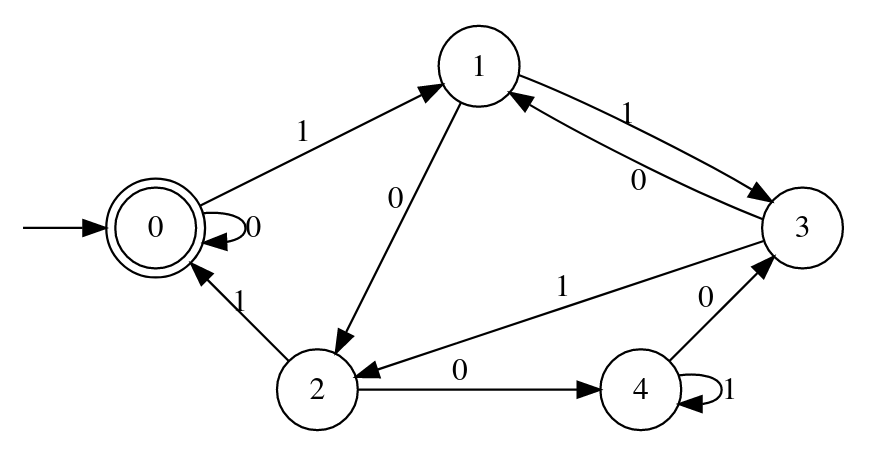
\includegraphics[width=3in]{images/gv/mc02-fa-ex3.png}
  \end{center}

  \pause

  If string $x$ and $y$ reach the same state in a DFA, for any string
  $z$, both $xz$ and $yz$ must reach the same state. \pause

  In other words, a DFA accepts $xz$ iff it accepts $yz$.

}

\frame{
  \frametitle{Distinguishing suffixes}

  Consider language $L=  \{ \czero^n\cone^n \;|\; n\geq 0 \}$.

  Consider $x=\czero$ and $y=\czero\czero$.  Consider suffix $z=\cone\cone$.

  \pause
  
  We have that
  \[
  xz=\czero{\color{red}\cone\cone} \not\in L,
  \]
  but
  \[
  yz=\czero\czero{\color{red}\cone\cone} \in L.
  \]

  \pause 

  What can you say about a DFA $M$ such that $L(M)=L$?

  \pause

  \begin{block}{Definition}
    For strings $x$ and $y$, string $z$ is a {\color{red}\bf
      distinguishing suffix} with respect to $L$ if exactly one of
    $xz$ and $yz$ is in $L$.
  \end{block}

}

\frame{
  \frametitle{Fooling sets}

  A {\color{red}\bf fooling set} for a language $L$ is set $F$ of
  strings such that every pair of strings in $F$ has a distinguishing
  suffix.

  \vspace{0.1in}
  
  {\bf Example:} The set $\{\czero, \czero\czero, \czero\czero\czero \}$ is a
  fooling set for $L= \{ \czero^n\cone^n \;|\; n\geq 0 \}$.

  \vspace{1.5in}
}

\frame{

  \frametitle{A large fooling set}

  \begin{lemma}
    The set $\{\czero^n \;|\; n\geq 0 \}$ is a fooling set for $L= \{
    \czero^n\cone^n \;|\; n\geq 0 \}$.
  \end{lemma}
  \begin{proof}
    \vspace{2in}
  \end{proof}
    
}

\frame{

  \begin{block}{Observation}
    If language $L$ has an infinite fooling set, $L$ is not regular
  \end{block}

  \pause

  \begin{lemma}
    Language $L= \{ \czero^n\cone^n \;|\; n\geq 0 \}$ is not regular.
  \end{lemma}
  \begin{proof}
    We previously establish that the set $F=\{\czero^n \;|\; n\geq 0
    \}$ is a fooling set for $L$.

    Since $F$ has infinite size, from the observation, we know that
    $L$ is not regular.
  \end{proof}
    

}

\frame{

  \begin{lemma}
    For $\Sigma=\{\czero,\cone\}$, the language $L=\{ ww^R \;|\;
    w\in\Sigma^* \}$ is not regular.
  \end{lemma}
  \begin{proof}
    \vspace{2in}
  \end{proof}
  
}

\frame{
  \frametitle{$L=\{ 0^{2^n} \;|\; n\geq 0\}$: Proof 1}

  \begin{lemma}
    For $\Sigma=\{\czero\}$, the language $L=\{ 0^{2^n} \;|\; n\geq 0
    \}$ is not regular.
  \end{lemma}
  \begin{proof}
    \vspace{2in}
  \end{proof}
  
}

\frame{
  \frametitle{$L=\{ 0^{2^n} \;|\; n\geq 0\}$: Proof 2}

  \begin{lemma}
    For $\Sigma=\{\czero\}$, the language $L=\{ 0^{2^n} \;|\; n\geq 0
    \}$ is not regular.
  \end{lemma}
  \begin{proof}
    \vspace{2in}
  \end{proof}
  
}

\frame{
  \frametitle{$L=\{ 0^{2^n} \;|\; n\geq 0\}$: Proof 3}

  \begin{lemma}
    For $\Sigma=\{\czero\}$, the language $L=\{ 0^{2^n} \;|\; n\geq 0
    \}$ is not regular.
  \end{lemma}
  \begin{proof}
    \vspace{2in}
  \end{proof}
  
}
\frame{
  \frametitle{$L=\{ 0^{p} \;|\; \mbox{$p$ is prime}\}$: Proof 1}

  \begin{lemma}
    For $\Sigma=\{\czero\}$, the language $L=\{ 0^{p} \;|\; \mbox{$p$
      is prime} \}$ is not regular.
  \end{lemma}
  \begin{proof}
    \vspace{2in}
  \end{proof}
  
}

\frame{
  \frametitle{$L=\{ 0^{p} \;|\; \mbox{$p$ is prime}\}$: Proof 2}

  \begin{lemma}
    For $\Sigma=\{\czero\}$, the language $L=\{ 0^{p} \;|\; \mbox{$p$
      is prime} \}$ is not regular.
  \end{lemma}
  \begin{proof}
    \vspace{2in}
  \end{proof}
  
}
